% Options for packages loaded elsewhere
\PassOptionsToPackage{unicode}{hyperref}
\PassOptionsToPackage{hyphens}{url}
%
\documentclass[
]{book}
\usepackage{amsmath,amssymb}
\usepackage{iftex}
\ifPDFTeX
  \usepackage[T1]{fontenc}
  \usepackage[utf8]{inputenc}
  \usepackage{textcomp} % provide euro and other symbols
\else % if luatex or xetex
  \usepackage{unicode-math} % this also loads fontspec
  \defaultfontfeatures{Scale=MatchLowercase}
  \defaultfontfeatures[\rmfamily]{Ligatures=TeX,Scale=1}
\fi
\usepackage{lmodern}
\ifPDFTeX\else
  % xetex/luatex font selection
\fi
% Use upquote if available, for straight quotes in verbatim environments
\IfFileExists{upquote.sty}{\usepackage{upquote}}{}
\IfFileExists{microtype.sty}{% use microtype if available
  \usepackage[]{microtype}
  \UseMicrotypeSet[protrusion]{basicmath} % disable protrusion for tt fonts
}{}
\makeatletter
\@ifundefined{KOMAClassName}{% if non-KOMA class
  \IfFileExists{parskip.sty}{%
    \usepackage{parskip}
  }{% else
    \setlength{\parindent}{0pt}
    \setlength{\parskip}{6pt plus 2pt minus 1pt}}
}{% if KOMA class
  \KOMAoptions{parskip=half}}
\makeatother
\usepackage{xcolor}
\usepackage{color}
\usepackage{fancyvrb}
\newcommand{\VerbBar}{|}
\newcommand{\VERB}{\Verb[commandchars=\\\{\}]}
\DefineVerbatimEnvironment{Highlighting}{Verbatim}{commandchars=\\\{\}}
% Add ',fontsize=\small' for more characters per line
\usepackage{framed}
\definecolor{shadecolor}{RGB}{248,248,248}
\newenvironment{Shaded}{\begin{snugshade}}{\end{snugshade}}
\newcommand{\AlertTok}[1]{\textcolor[rgb]{0.94,0.16,0.16}{#1}}
\newcommand{\AnnotationTok}[1]{\textcolor[rgb]{0.56,0.35,0.01}{\textbf{\textit{#1}}}}
\newcommand{\AttributeTok}[1]{\textcolor[rgb]{0.13,0.29,0.53}{#1}}
\newcommand{\BaseNTok}[1]{\textcolor[rgb]{0.00,0.00,0.81}{#1}}
\newcommand{\BuiltInTok}[1]{#1}
\newcommand{\CharTok}[1]{\textcolor[rgb]{0.31,0.60,0.02}{#1}}
\newcommand{\CommentTok}[1]{\textcolor[rgb]{0.56,0.35,0.01}{\textit{#1}}}
\newcommand{\CommentVarTok}[1]{\textcolor[rgb]{0.56,0.35,0.01}{\textbf{\textit{#1}}}}
\newcommand{\ConstantTok}[1]{\textcolor[rgb]{0.56,0.35,0.01}{#1}}
\newcommand{\ControlFlowTok}[1]{\textcolor[rgb]{0.13,0.29,0.53}{\textbf{#1}}}
\newcommand{\DataTypeTok}[1]{\textcolor[rgb]{0.13,0.29,0.53}{#1}}
\newcommand{\DecValTok}[1]{\textcolor[rgb]{0.00,0.00,0.81}{#1}}
\newcommand{\DocumentationTok}[1]{\textcolor[rgb]{0.56,0.35,0.01}{\textbf{\textit{#1}}}}
\newcommand{\ErrorTok}[1]{\textcolor[rgb]{0.64,0.00,0.00}{\textbf{#1}}}
\newcommand{\ExtensionTok}[1]{#1}
\newcommand{\FloatTok}[1]{\textcolor[rgb]{0.00,0.00,0.81}{#1}}
\newcommand{\FunctionTok}[1]{\textcolor[rgb]{0.13,0.29,0.53}{\textbf{#1}}}
\newcommand{\ImportTok}[1]{#1}
\newcommand{\InformationTok}[1]{\textcolor[rgb]{0.56,0.35,0.01}{\textbf{\textit{#1}}}}
\newcommand{\KeywordTok}[1]{\textcolor[rgb]{0.13,0.29,0.53}{\textbf{#1}}}
\newcommand{\NormalTok}[1]{#1}
\newcommand{\OperatorTok}[1]{\textcolor[rgb]{0.81,0.36,0.00}{\textbf{#1}}}
\newcommand{\OtherTok}[1]{\textcolor[rgb]{0.56,0.35,0.01}{#1}}
\newcommand{\PreprocessorTok}[1]{\textcolor[rgb]{0.56,0.35,0.01}{\textit{#1}}}
\newcommand{\RegionMarkerTok}[1]{#1}
\newcommand{\SpecialCharTok}[1]{\textcolor[rgb]{0.81,0.36,0.00}{\textbf{#1}}}
\newcommand{\SpecialStringTok}[1]{\textcolor[rgb]{0.31,0.60,0.02}{#1}}
\newcommand{\StringTok}[1]{\textcolor[rgb]{0.31,0.60,0.02}{#1}}
\newcommand{\VariableTok}[1]{\textcolor[rgb]{0.00,0.00,0.00}{#1}}
\newcommand{\VerbatimStringTok}[1]{\textcolor[rgb]{0.31,0.60,0.02}{#1}}
\newcommand{\WarningTok}[1]{\textcolor[rgb]{0.56,0.35,0.01}{\textbf{\textit{#1}}}}
\usepackage{longtable,booktabs,array}
\usepackage{calc} % for calculating minipage widths
% Correct order of tables after \paragraph or \subparagraph
\usepackage{etoolbox}
\makeatletter
\patchcmd\longtable{\par}{\if@noskipsec\mbox{}\fi\par}{}{}
\makeatother
% Allow footnotes in longtable head/foot
\IfFileExists{footnotehyper.sty}{\usepackage{footnotehyper}}{\usepackage{footnote}}
\makesavenoteenv{longtable}
\usepackage{graphicx}
\makeatletter
\def\maxwidth{\ifdim\Gin@nat@width>\linewidth\linewidth\else\Gin@nat@width\fi}
\def\maxheight{\ifdim\Gin@nat@height>\textheight\textheight\else\Gin@nat@height\fi}
\makeatother
% Scale images if necessary, so that they will not overflow the page
% margins by default, and it is still possible to overwrite the defaults
% using explicit options in \includegraphics[width, height, ...]{}
\setkeys{Gin}{width=\maxwidth,height=\maxheight,keepaspectratio}
% Set default figure placement to htbp
\makeatletter
\def\fps@figure{htbp}
\makeatother
\setlength{\emergencystretch}{3em} % prevent overfull lines
\providecommand{\tightlist}{%
  \setlength{\itemsep}{0pt}\setlength{\parskip}{0pt}}
\setcounter{secnumdepth}{-\maxdimen} % remove section numbering
\newlength{\cslhangindent}
\setlength{\cslhangindent}{1.5em}
\newlength{\csllabelwidth}
\setlength{\csllabelwidth}{3em}
\newlength{\cslentryspacingunit} % times entry-spacing
\setlength{\cslentryspacingunit}{\parskip}
\newenvironment{CSLReferences}[2] % #1 hanging-ident, #2 entry spacing
 {% don't indent paragraphs
  \setlength{\parindent}{0pt}
  % turn on hanging indent if param 1 is 1
  \ifodd #1
  \let\oldpar\par
  \def\par{\hangindent=\cslhangindent\oldpar}
  \fi
  % set entry spacing
  \setlength{\parskip}{#2\cslentryspacingunit}
 }%
 {}
\usepackage{calc}
\newcommand{\CSLBlock}[1]{#1\hfill\break}
\newcommand{\CSLLeftMargin}[1]{\parbox[t]{\csllabelwidth}{#1}}
\newcommand{\CSLRightInline}[1]{\parbox[t]{\linewidth - \csllabelwidth}{#1}\break}
\newcommand{\CSLIndent}[1]{\hspace{\cslhangindent}#1}
\ifLuaTeX
  \usepackage{selnolig}  % disable illegal ligatures
\fi
\IfFileExists{bookmark.sty}{\usepackage{bookmark}}{\usepackage{hyperref}}
\IfFileExists{xurl.sty}{\usepackage{xurl}}{} % add URL line breaks if available
\urlstyle{same}
\hypersetup{
  pdftitle={ԱՆԱԼՈԳԱՅԻՆ ԻՆՏԵԳՐԱԼ ՍԽԵՄԱՆԵՐԻ ՆԱԽԱԳԾՈՒՄ։},
  pdfauthor={Հեղինակներ՝ Մարիամ Հակոբյան, Նարինե Գալստյան, Երանուհի Զուլալյան, Արմեն Համբարյան, Վարդան Անատոմյան։   Ղեկավարներ՝ Մերի Մարգարյան, Արթուր Բայբուրդյան։},
  hidelinks,
  pdfcreator={LaTeX via pandoc}}

\title{ԱՆԱԼՈԳԱՅԻՆ ԻՆՏԵԳՐԱԼ ՍԽԵՄԱՆԵՐԻ ՆԱԽԱԳԾՈՒՄ։}
\author{\textbf{Հեղինակներ՝} Մարիամ Հակոբյան, Նարինե Գալստյան, Երանուհի
Զուլալյան, Արմեն Համբարյան, Վարդան Անատոմյան։ \textbf{Ղեկավարներ՝} Մերի
Մարգարյան, Արթուր Բայբուրդյան։}
\date{2023-12-04}

\begin{document}
\frontmatter
\maketitle

\mainmatter
\hypertarget{ux576ux565ux580ux561ux56eux578ux582ux569ux575ux578ux582ux576}{%
\chapter{ՆԵՐԱԾՈՒԹՅՈՒՆ։}\label{ux576ux565ux580ux561ux56eux578ux582ux569ux575ux578ux582ux576}}

Նախքան \textbf{օպեռացիոն ուժեղարարների}բնութագրիչ մեծությունների,
կառուցվածքի, նախագծման փուլերի, դրանց առանձնահատկությունների մասին
խոսելը ներածական մասը կնվիրենք դաշտային տռանզիստորների կառուցվածքի,
աշխատանքային ռեժիմների Վոլտ֊Ամպեռային \textbf{«ՎԱԲ»} բնութագրի համառոտ
ներկայացմամը։

\hypertarget{ux574ux585ux56f-ux574ux565ux57fux561ux572-ux585ux584ux57dux56bux564-ux56fux56bux57dux561ux570ux561ux572ux578ux580ux564ux56bux579-ux57fux57cux561ux576ux566ux56bux57dux57fux578ux580ux576ux565ux580}{%
\section{ՄՕԿ Մետաղ օքսիդ կիսահաղորդիչ
տռանզիստորներ։}\label{ux574ux585ux56f-ux574ux565ux57fux561ux572-ux585ux584ux57dux56bux564-ux56fux56bux57dux561ux570ux561ux572ux578ux580ux564ux56bux579-ux57fux57cux561ux576ux566ux56bux57dux57fux578ux580ux576ux565ux580}}

\begin{figure}

{\centering 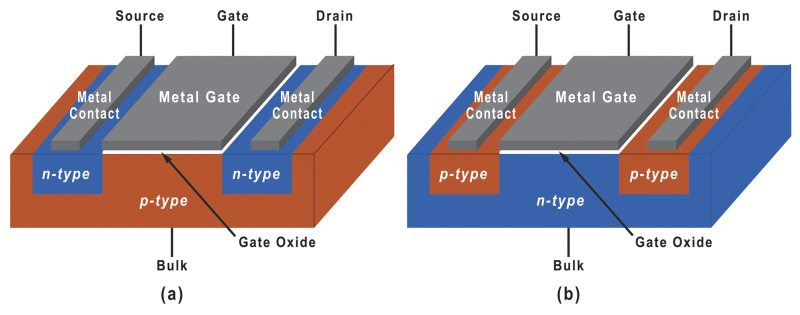
\includegraphics[width=1\linewidth]{imige/mostex} 

}

\caption{...}\label{fig:unnamed-chunk-1}
\end{figure}

Նկարում պատկերված են \textbf{ՆՄՕԿ} և \textbf{ՊՄՈԿ} տրանզիստորների
պարզեցված կառուցվածքը։ Ինչպես երևում է նկարից սարքերը սիմետրիկ էն փականի
նկատմամբ, որը պատճառներից մեկն է լայնամաշտաբ կիռառման, քանի որ
հեշտացնում է արտադրական պռոցեսները իտարբերություն երկբևեռ
տրանզիստորների։ Ինտեգրալ սխեմաներ պատրաստելուց վերցնում են P տիպի
կիսահաղորդիչ հարթակ «substrate»: ՊՄՕԿ տռանզիստորներ ստանալու համար
տարբեր եղանակներով հարթակի մեջ ներդնում են N տիպի իմպլանտ։

Աշխատանքի սկզբունքը ուսունմասիրելու համար դիտարկենք ՆՄՕԿ տրանզիստորը։
տրանզիստորի աշխատանքի համար իրականում անհրաժեշտ է ևս մեկ ելուս որպիսի
հարթակին պոտենցիալ հաղորդի։ Հարթակից ակունք և ըմբիչ հոսանք չանցնելու
համար պետկ է հարթակը ունենա ավելի ցածր պոտենցիալ։ Պարզության համար
ենթադրենք հարթակը և ակունքը միացված են իրար։ Ինչպես երևում է նկարից
փականը և հարթակը առանձնացված են օքսիդով այս կառուցվածքը իրենից
ներկայացնում կոնդեսատոր։

\hypertarget{ux577ux565ux574ux561ux575ux56bux576-treshold-ux56cux561ux580ux578ux582ux574}{%
\section{Շեմային «treshold»
լարում։}\label{ux577ux565ux574ux561ux575ux56bux576-treshold-ux56cux561ux580ux578ux582ux574}}

\begin{figure}

{\centering 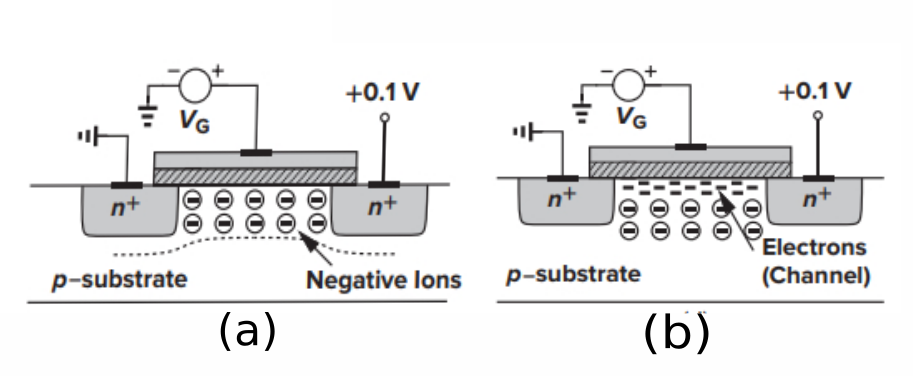
\includegraphics[width=1\linewidth]{imige/th} 

}

\caption{...}\label{fig:unnamed-chunk-2}
\end{figure}

Դիտարկենք նկարում պատկերված արտաքին լարումներին միացված ՆՄՈԿ֊ը։ Երբ
փականի պոտենցիալը հարթակի նկատմամբ մեծանում է \(\pmb{\varphi>0}\)
հարթակի ազատ լիցքակիրները խոռոչները սկսում են վանվել ներքև թողնելով
բացասական իոններ ստեղծվում է աղքատացված տիրույթ։ Այսպիսով որքան մեծանա
\(\pmb{\varphi}\)֊ն այնքան ավելի կհաստանա աղքատացման տիրույթը հետևաբար
խոռոչների կոնցենտրացիան հարթակի ներքևում ավելի կմեծանա։
\(\pmb{\varphi}\)֊ի բավարար մեծ արժեքի դեպքում օքսիդի տակ սկսում է իհայտ
գալ ազատ էլեկտրոններ որոնց մի մասը ակունքիցից են հոսել իսկ մի մասը
հարթակից։ Այսպիսով ակունքի և ըմբիչի միջև առաջանում է հոսքուղի։ այս
երևույթը հաճախ անվանում են նաև կիսահաղորդչի տիպի շրջում։

\textbf{\(V_{gs}\)֊ի այն մինիմալ լարումը որի դեպքում առաջանում է
հոսքուղի «տեղի է ունենում ինվերսիա» կոչվում է շեմային լարում:}

\begin{equation} 
  V_{TH} = 𝜱_{MS} + 2 𝜱_F + \frac{G_{dep}}{C_ox}
  (\#eq:binom)
\end{equation}

Որտեղ՝

\begin{itemize}
\tightlist
\item
  \(𝜱_{MS}\)֊ը հարթակի և փականի աշխատանքային ֆունկցիաների տարբերությունն
  է։
\item
  \(𝜱_F = \frac{kT}{q} \ln{\frac{N_{sub}}{n_i}}\)

  \begin{itemize}
  \tightlist
  \item
    \(k\)֊ն Բելցմանի հաստատուն։
  \item
    \(N_{sub}\)֊ը հարթակի լիցքակիրների կոնցետրացիան \textbf{«doping
    density»}:
  \item
    \(n_i\)֊ը մաքուր կիսահաղորդիչ հարթակի լիցքակիրների կոնցետրացիան
    \textbf{«udoping density»}:
  \end{itemize}
\item
  \(C_{ox}\)֊ը միաոր մակերես ունեցող հաթակ օքսիդ ըմբիչ կոնդեսատորի
  ունակությունն է։
\item
  \(Q_dep\)֊ը աղքատացման տիրույթի իոնների լիցքն է։
\end{itemize}

Ներկայումս երբ տրանզիստորների չափերը համենատելի են ատոմի չափերին շատ
դժվար է տալ բանաձև ոչ միայն շեմային լարման այլ նաև ՎԱԲ֊ի և այլ
բնութագրերի համար, այդ պատճառով պարամետրերը հաճախ \textbf{գնահատում} են
օգտվելով վիճակագրական մեթոդներից։

\hypertarget{ux57eux578ux56cux57fux561ux574ux57aux565ux57cux561ux575ux56bux576-ux562ux576ux578ux582ux569ux561ux563ux56bux580ux568}{%
\section{Վոլտ֊Ամպեռային
բնութագիրը։}\label{ux57eux578ux56cux57fux561ux574ux57aux565ux57cux561ux575ux56bux576-ux562ux576ux578ux582ux569ux561ux563ux56bux580ux568}}

ՄՈԿ տրանզիստորի վոլտ֊Ամպեռային բնութագրի մասին խոսելիս կուզենաինք նշել
որ, երբ փականի պոտենցիալը գերազանցում է շեմային լարումը ըմբիչով կարող է
հոսանք անցնել նշանակում է՝ տրանզիստորը բաց է սակայն փականով հոսանք չի
անցնում։

Դիտարկենք նկարում պատկերված արտաքին լարումներին միացված երկու դեպքերը։

\begin{figure}

{\centering 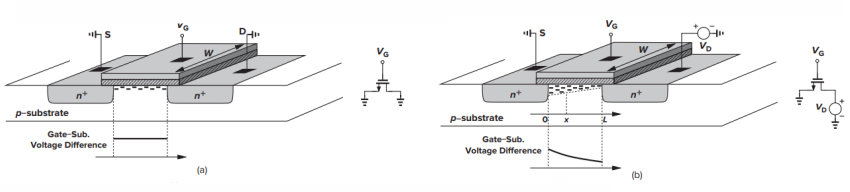
\includegraphics[width=1\linewidth]{imige/va} 

}

\caption{...}\label{fig:unnamed-chunk-3}
\end{figure}

\begin{blackbox}

\begin{lf}

\begin{center}
Երբ ակունքի և ըմբիչի պոտենցիալները իրար հավասար են՝ \begin{align}  
  Q_d = WC_{ox}(V_{GS} - V_{TH})
\end{align}

\end{center}

\end{lf}

\begin{rig}

\begin{center}
Երբ \(V_{DS>0}\) հոսքուղու որևէ X կետում՝

\begin{align} 
  Q_d = WC_{ox}(V_{GS} - V_{TH})
\end{align}

\end{center}

\end{rig}

\end{blackbox}

Այժմ ենթադրենք ունենք N տիպի բավական երկար կիսահաղորդիչ որը տեղադրված է
համասեռ մեկ միաոր էլ․ դաշտում։ Ակնհայտ լիցքակիրները կսկսեն արագանալ
սակայն տեղի են ունենում բախումներ այդ պատճառուվ որոշները կանգ կառնեն և
նորից կսկսեն արագանալ որոշները կարող է ընդհանրապես հանդիպեն խոռոչի և
զբաղեցնեն ազատ տեղը։ Այսպիսով որպիսի կարողանանք բնութագրենք շարժումը
ներմուծենք լիցքի շարժողականություն մեծությունը, որը միջինացված արժեք է և
ցուից է տալիս թե միջինում ինչ արագությամբ է շարժվում լիցքակիրը արտաքին
էլ․ դաշտի ազդեցության տակ \(μ_n = \frac{V}{E}\)։

Երբ հայտնի է ազատ լիցքակիրների բաշխվածությունը օգտվելով էլ․ հոսանքի
սահմանումից կստանանք՝

\begin{equation} 
  I_{D} = μ_n C_{ox} \frac{W}{L}[(V_{GS} - V_{TH})V_{DS} - \frac{1}{2}V_{DS}^2]
  (\#eq:align)
\end{equation}

\hypertarget{ux578ux582ux56aux565ux572ux561ux580ux561ux580ux576ux565ux580}{%
\chapter{ՈՒժեղարարներ}\label{ux578ux582ux56aux565ux572ux561ux580ux561ux580ux576ux565ux580}}

\hypertarget{ux574ux585ux57d-ux574ux565ux57fux561ux572-ux585ux584ux57dux56bux57f-ux56fux56bux57dux561ux570ux561ux572ux578ux580ux564ux56bux579-ux57dux561ux580ux584ux565ux580}{%
\section{ՄՕՍ մետաղ օքսիտ կիսահաղորդիչ
սարքեր։}\label{ux574ux585ux57d-ux574ux565ux57fux561ux572-ux585ux584ux57dux56bux57f-ux56fux56bux57dux561ux570ux561ux572ux578ux580ux564ux56bux579-ux57dux561ux580ux584ux565ux580}}

\begin{Shaded}
\begin{Highlighting}[]
\ImportTok{import}\NormalTok{ numpy }\ImportTok{as}\NormalTok{ np}
\ImportTok{import}\NormalTok{ matplotlib.pyplot }\ImportTok{as}\NormalTok{ plt}
\NormalTok{x }\OperatorTok{=}\NormalTok{ np.linspace(}\OperatorTok{{-}}\NormalTok{np.pi , np.pi, }\DecValTok{100}\NormalTok{)}
\NormalTok{y }\OperatorTok{=}\NormalTok{ np.sin(x)}
\NormalTok{plt.plot(x , y)}
\NormalTok{plt.show()}
\end{Highlighting}
\end{Shaded}

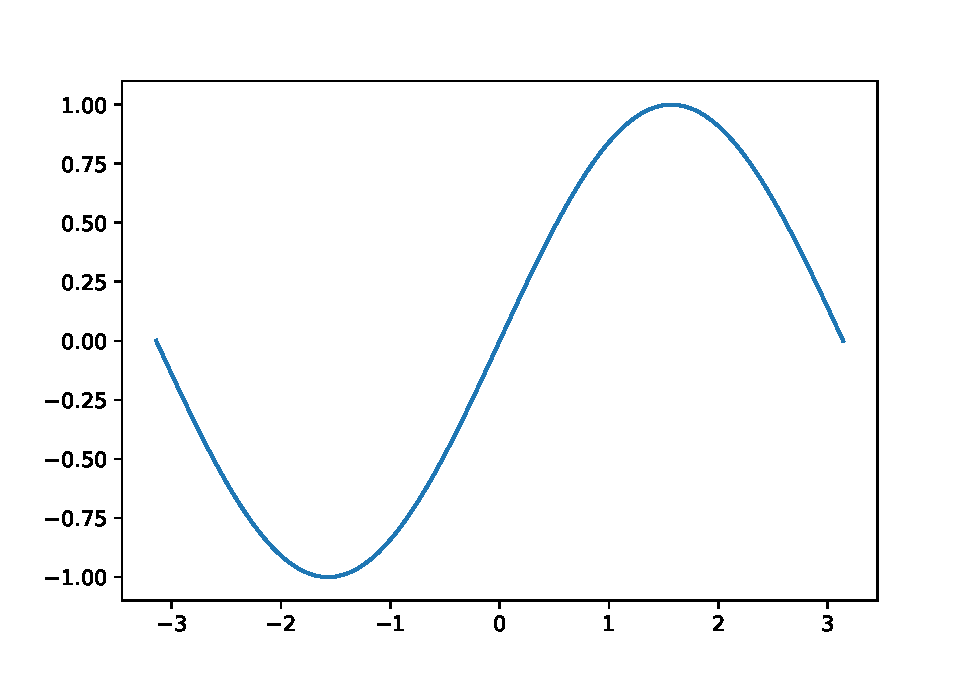
\includegraphics{_main_files/figure-latex/unnamed-chunk-5-1.pdf}

\hypertarget{cross}{%
\chapter{Cross-references}\label{cross}}

Cross-references make it easier for your readers to find and link to
elements in your book.

\hypertarget{chapters-and-sub-chapters}{%
\section{Chapters and sub-chapters}\label{chapters-and-sub-chapters}}

There are two steps to cross-reference any heading:

\begin{enumerate}
\def\labelenumi{\arabic{enumi}.}
\tightlist
\item
  Label the heading: \texttt{\#\ Hello\ world\ \{\#nice-label\}}.

  \begin{itemize}
  \tightlist
  \item
    Leave the label off if you like the automated heading generated
    based on your heading title: for example, \texttt{\#\ Hello\ world}
    = \texttt{\#\ Hello\ world\ \{\#hello-world\}}.
  \item
    To label an un-numbered heading, use:
    \texttt{\#\ Hello\ world\ \{-\#nice-label\}} or
    \texttt{\{\#\ Hello\ world\ .unnumbered\}}.
  \end{itemize}
\item
  Next, reference the labeled heading anywhere in the text using
  \texttt{\textbackslash{}@ref(nice-label)}; for example, please see
  Chapter @ref(cross).

  \begin{itemize}
  \tightlist
  \item
    If you prefer text as the link instead of a numbered reference use:
    \protect\hyperlink{cross}{any text you want can go here}.
  \end{itemize}
\end{enumerate}

\hypertarget{captioned-figures-and-tables}{%
\section{Captioned figures and
tables}\label{captioned-figures-and-tables}}

Figures and tables \emph{with captions} can also be cross-referenced
from elsewhere in your book using
\texttt{\textbackslash{}@ref(fig:chunk-label)} and
\texttt{\textbackslash{}@ref(tab:chunk-label)}, respectively.

See Figure @ref(fig:nice-fig).

\begin{Shaded}
\begin{Highlighting}[]
\FunctionTok{par}\NormalTok{(}\AttributeTok{mar =} \FunctionTok{c}\NormalTok{(}\DecValTok{4}\NormalTok{, }\DecValTok{4}\NormalTok{, .}\DecValTok{1}\NormalTok{, .}\DecValTok{1}\NormalTok{))}
\FunctionTok{plot}\NormalTok{(pressure, }\AttributeTok{type =} \StringTok{\textquotesingle{}b\textquotesingle{}}\NormalTok{, }\AttributeTok{pch =} \DecValTok{19}\NormalTok{)}
\end{Highlighting}
\end{Shaded}

\begin{figure}

{\centering 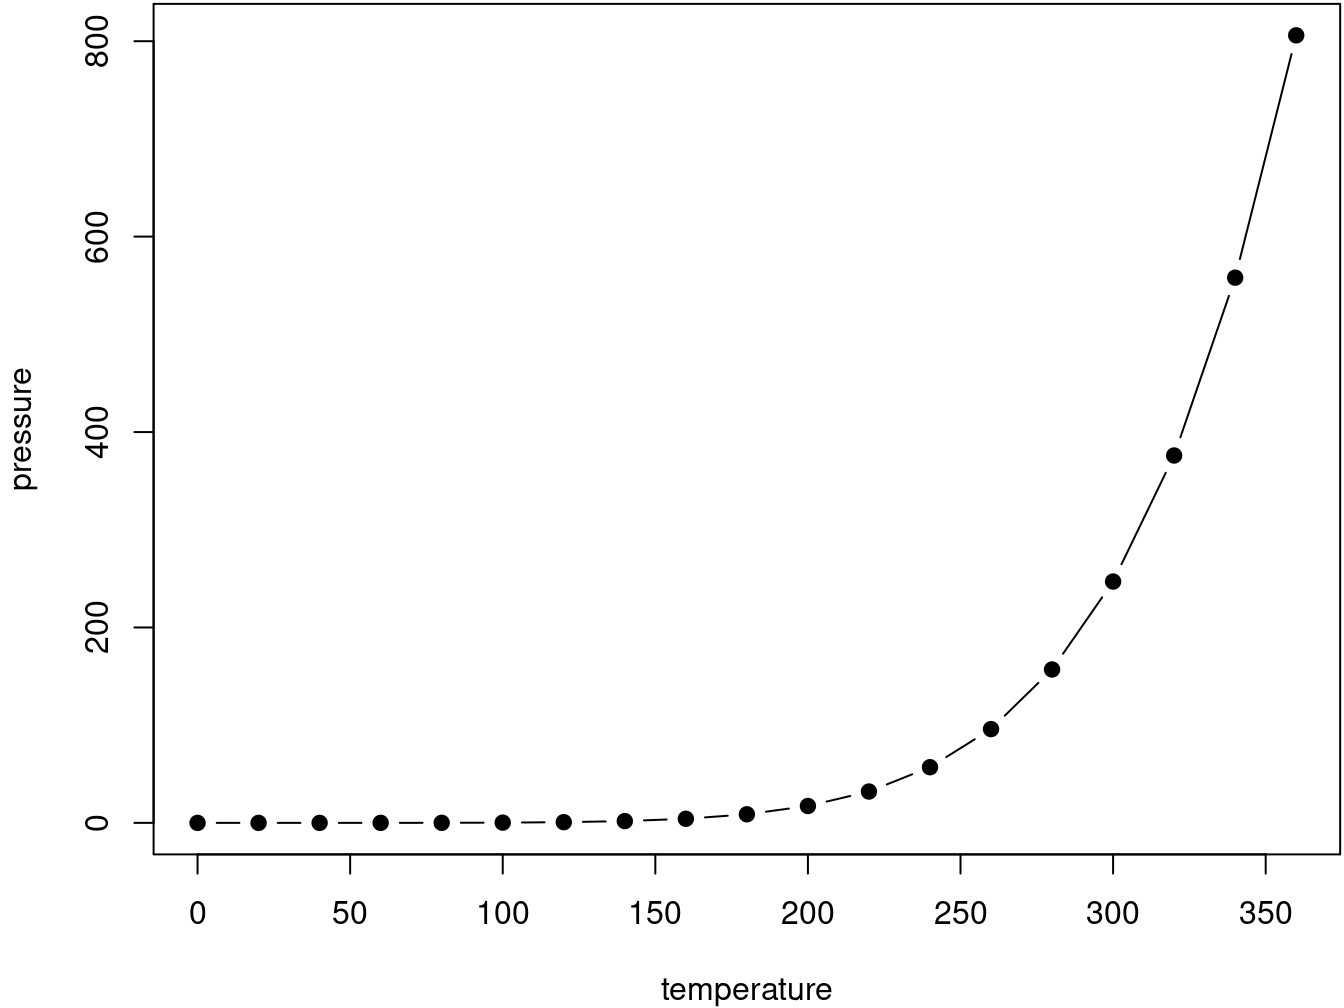
\includegraphics[width=0.8\linewidth]{_main_files/figure-latex/nice-fig-1} 

}

\caption{Here is a nice figure!}\label{fig:nice-fig}
\end{figure}

Don't miss Table @ref(tab:nice-tab).

\begin{Shaded}
\begin{Highlighting}[]
\NormalTok{knitr}\SpecialCharTok{::}\FunctionTok{kable}\NormalTok{(}
  \FunctionTok{head}\NormalTok{(pressure, }\DecValTok{10}\NormalTok{), }\AttributeTok{caption =} \StringTok{\textquotesingle{}Here is a nice table!\textquotesingle{}}\NormalTok{,}
  \AttributeTok{booktabs =} \ConstantTok{TRUE}
\NormalTok{)}
\end{Highlighting}
\end{Shaded}

\begin{longtable}[]{@{}rr@{}}
\caption{Here is a nice table!}\tabularnewline
\toprule\noalign{}
temperature & pressure \\
\midrule\noalign{}
\endfirsthead
\toprule\noalign{}
temperature & pressure \\
\midrule\noalign{}
\endhead
\bottomrule\noalign{}
\endlastfoot
0 & 0.0002 \\
20 & 0.0012 \\
40 & 0.0060 \\
60 & 0.0300 \\
80 & 0.0900 \\
100 & 0.2700 \\
120 & 0.7500 \\
140 & 1.8500 \\
160 & 4.2000 \\
180 & 8.8000 \\
\end{longtable}

\hypertarget{parts}{%
\chapter{Parts}\label{parts}}

You can add parts to organize one or more book chapters together. Parts
can be inserted at the top of an .Rmd file, before the first-level
chapter heading in that same file.

Add a numbered part: \texttt{\#\ (PART)\ Act\ one\ \{-\}} (followed by
\texttt{\#\ A\ chapter})

Add an unnumbered part:
\texttt{\#\ (PART\textbackslash{}*)\ Act\ one\ \{-\}} (followed by
\texttt{\#\ A\ chapter})

Add an appendix as a special kind of un-numbered part:
\texttt{\#\ (APPENDIX)\ Other\ stuff\ \{-\}} (followed by
\texttt{\#\ A\ chapter}). Chapters in an appendix are prepended with
letters instead of numbers.

\hypertarget{footnotes-and-citations}{%
\chapter{Footnotes and citations}\label{footnotes-and-citations}}

\hypertarget{footnotes}{%
\section{Footnotes}\label{footnotes}}

Footnotes are put inside the square brackets after a caret
\texttt{\^{}{[}{]}}. Like this one \footnote{This is a footnote.}.

\hypertarget{citations}{%
\section{Citations}\label{citations}}

Reference items in your bibliography file(s) using \texttt{@key}.

For example, we are using the \textbf{bookdown} package
(\protect\hyperlink{ref-R-bookdown}{Xie 2023}) (check out the last code
chunk in index.Rmd to see how this citation key was added) in this
sample book, which was built on top of R Markdown and \textbf{knitr}
(\protect\hyperlink{ref-xie2015}{Xie 2015}) (this citation was added
manually in an external file book.bib). Note that the \texttt{.bib}
files need to be listed in the index.Rmd with the YAML
\texttt{bibliography} key.

The RStudio Visual Markdown Editor can also make it easier to insert
citations:
\url{https://rstudio.github.io/visual-markdown-editing/\#/citations}

\hypertarget{blocks}{%
\chapter{Blocks}\label{blocks}}

\hypertarget{equations}{%
\section{Equations}\label{equations}}

Here is an equation.

\begin{equation} 
  f\left(k\right) = \binom{n}{k} p^k\left(1-p\right)^{n-k}
  (\#eq:binom)
\end{equation}

You may refer to using \texttt{\textbackslash{}@ref(eq:binom)}, like see
Equation @ref(eq:binom).

\hypertarget{theorems-and-proofs}{%
\section{Theorems and proofs}\label{theorems-and-proofs}}

Labeled theorems can be referenced in text using
\texttt{\textbackslash{}@ref(thm:tri)}, for example, check out this
smart theorem @ref(thm:tri).

\leavevmode\vadjust pre{\hypertarget{tri}{}}%
For a right triangle, if \(c\) denotes the \emph{length} of the
hypotenuse and \(a\) and \(b\) denote the lengths of the \textbf{other}
two sides, we have \[a^2 + b^2 = c^2\]

Read more here
\url{https://bookdown.org/yihui/bookdown/markdown-extensions-by-bookdown.html}.

\hypertarget{callout-blocks}{%
\section{Callout blocks}\label{callout-blocks}}

The R Markdown Cookbook provides more help on how to use custom blocks
to design your own callouts:
\url{https://bookdown.org/yihui/rmarkdown-cookbook/custom-blocks.html}

\hypertarget{sharing-your-book}{%
\chapter{Sharing your book}\label{sharing-your-book}}

\hypertarget{publishing}{%
\section{Publishing}\label{publishing}}

HTML books can be published online, see:
\url{https://bookdown.org/yihui/bookdown/publishing.html}

\hypertarget{pages}{%
\section{404 pages}\label{pages}}

By default, users will be directed to a 404 page if they try to access a
webpage that cannot be found. If you'd like to customize your 404 page
instead of using the default, you may add either a \texttt{\_404.Rmd} or
\texttt{\_404.md} file to your project root and use code and/or Markdown
syntax.

\hypertarget{metadata-for-sharing}{%
\section{Metadata for sharing}\label{metadata-for-sharing}}

Bookdown HTML books will provide HTML metadata for social sharing on
platforms like Twitter, Facebook, and LinkedIn, using information you
provide in the \texttt{index.Rmd} YAML. To setup, set the \texttt{url}
for your book and the path to your \texttt{cover-image} file. Your
book's \texttt{title} and \texttt{description} are also used.

This \texttt{gitbook} uses the same social sharing data across all
chapters in your book- all links shared will look the same.

Specify your book's source repository on GitHub using the \texttt{edit}
key under the configuration options in the \texttt{\_output.yml} file,
which allows users to suggest an edit by linking to a chapter's source
file.

Read more about the features of this output format here:

\url{https://pkgs.rstudio.com/bookdown/reference/gitbook.html}

Or use:

\begin{Shaded}
\begin{Highlighting}[]
\NormalTok{?bookdown}\SpecialCharTok{::}\NormalTok{gitbook}
\end{Highlighting}
\end{Shaded}

\hypertarget{refs}{}
\begin{CSLReferences}{1}{0}
\leavevmode\vadjust pre{\hypertarget{ref-xie2015}{}}%
Xie, Yihui. 2015. \emph{Dynamic Documents with {R} and Knitr}. 2nd ed.
Boca Raton, Florida: Chapman; Hall/CRC. \url{http://yihui.org/knitr/}.

\leavevmode\vadjust pre{\hypertarget{ref-R-bookdown}{}}%
---------. 2023. \emph{Bookdown: Authoring Books and Technical Documents
with r Markdown}. \url{https://github.com/rstudio/bookdown}.

\end{CSLReferences}

\backmatter
\end{document}
